\documentclass[12pt]{article}

\usepackage{amsfonts,amssymb,amsmath}
\usepackage{setspace,achicago,graphicx,url}



\usepackage[top=.9in, bottom=.9in, left=.9in , right=.9in,letterpaper]{geometry}



%For accepting graphs
\usepackage{graphicx}

% to allow links to the reply
\usepackage{xr-hyper}
\externaldocument[M-]{prohibitorum}
\externaldocument[O-]{prohibitorum-appendix}

\parskip5mm


\begin{document}

\hfill September 2022

\textbf{MS2022 – 443-1: “Catholic Censorship and the Demise of Knowledge Production in
Early Modern Italy”, by Fabio Blasutto and David de la Croix}

\textbf{Response to Referee 2}


We are  grateful to Referee 2 for their positive evaluation of our work – and
for providing numerous suggestions that, we believe, allowed us to improve substantially our
paper. Below, we detail how our revision deals with each of the issues raised by the Referee.
The referee's comments are in italics, followed by our point-to-point replies.

\textit{
1. I would find interesting to understand whether the channel the authors discuss, i.e. the effect of censorship
on agents’ choice between producing compliant and non-compliant publications, is totally new or has been
put forward previously by other scholars (e.g. by historians, etc…).
}


In other disciplines, scholars highlighted the role of self-censorship for sectoral choice.\footnote{For example, \citeN{gusdorf1971} wrote “Il fallait se soumettre ou se démettre, ou encore tricher à ses risques et périls.” These words mean that scientists in the $16^{th}$-century Italy had to choose between abandoning their work and continuing doing their research with the risk of being caught by the Roman Inquisition.} Our novel mechanism is that censorship decreases the relative quality of heretical ideas and this makes printers less likely to print heretical books. We formulated this mechanism to rationalize two novel facts: once censorship was introduced, censored authors were of better quality than non-censored authors, but this gap shrank over time, and the intensity of censorship decreased over time.


\textit{
2. Page 6: the authors “…count the number of publications, including different editions of the same work.”
Is this assumption relevant? What happens if different editions of the same work are not counted.
}

This point refers to what information is available in Worldcat for creating a measure of scholars' quality/notoriety. In this reply, we refer to the different measures available in Worldcat in italics. In the main text, we use the number of \textit{publications by} for our analysis, while \textit{publications} indeed counts different editions.
Two other measures are available: the \textit{number of works} aggregates \textit{publications by} and \textit{publications about} each scholar, but does not count the multiple editions of each work. The number of \textit{library holdings} today can be seen as a measure encompassing both output and recognition of its quality. All these measures include two dimensions, one related to written output and the other to citations. Note that citations are captured either by the publications about the scholar or by the reedition and translation of his/her impactful works.

We have written a new appendix (Appendix~\ref{O-app:robustdecline}) in which we provide the summary statistics using these and other measures to see if the decline of Italy is robust to the choice of the quality/notoriety measure. We were not surprised that it is indeed the case: the various WorldCat measures are very much correlated to each other (see the reply to the next point).



\textit{
3. One of the key assumptions is that the quality of the authors is proxied by the number of publications per
person. I am not one hundred percent convinced that the number of publications can be a good measure of
quality, especially if we refer to the quality of scholars as the capacity of producing radical innovations. Is
there any evidence that can be provided in support of this assumption? My common sense suggests this is
not true today, but maybe it was true in the past, or that I am wrong.
}

To address this point, we provide in a new Appendix  (Appendix~\ref{O-app:cor}) the correlation matrix of various measures of quality.

We conclude there that ``All the notoriety measures are highly correlated with each other, in particular when we use the rank correlation. In the main analysis, we opted for the variable ``publi by'' because it is the one which is the closest to our theoretical concept of books by an author. But we could have taken another one, all the computations in terms of quantiles would not be much affected.''



\textit{
4. Figure 2 presents the distribution of published authors by quality showing that in the first two periods the
censored authors were mostly those with more publications, and then censorship becomes more uniformly
distributed among authors in the other three periods. This effect could have a simple explanation: at the
beginning the Church has to set a censored apparatus and it is easier to focus on authors with large number
of publications, then over time this effect vanishes because. By the way, on Figure 2, it would be interesting
to see the distribution not in log.
}

Figure 1 in the new text (this Figure corresponds to Figure 2 in the older version of the manuscript) presents some new facts. We believe that a good model of censorship should reproduce them, but we do not pretend that they uniquely identify one theory. Other explanations, such as the one proposed by the referee, could also explain this figure. In the paper, we build confidence in our theory by showing its ability to quantitatively account for this and other facts.

Figure~\ref{fig:distrib} below shows the distribution not in logs. It is not very appealing because the top 5\% scholars have a very high number of publications, and the bottom 95\% is concentrated near the vertical axis.



\begin{figure}[htbp]

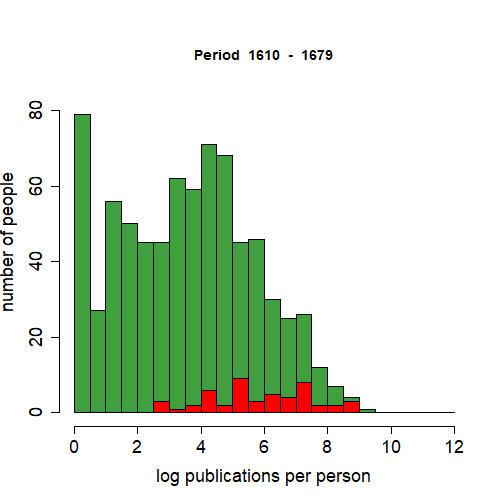
\includegraphics[width=.32\textwidth,trim=0cm 0cm 0cm 1cm, clip]{histo4Q.png}
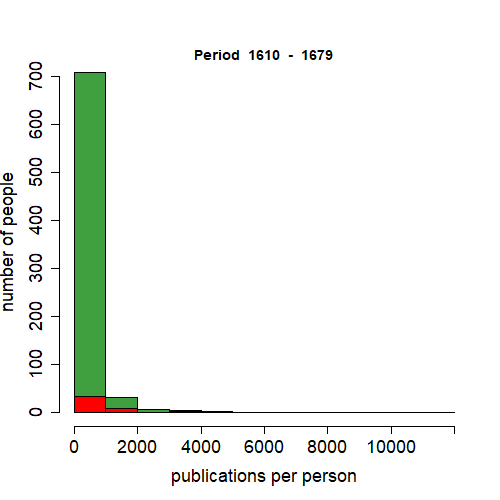
\includegraphics[width=.32\textwidth,trim=0cm 0cm 0cm 1cm, clip]{histo4Q-exp.png}

\caption{Distribution of published authors by quality. Period 4. In logs and in levels }\label{fig:distrib}

\end{figure}



\textit{
5. Even though I believe (at least part of) the idea that censorship had an important effect on the dynamic of
science in Italy, I wonder whether the effect about the different dynamics of publications in Italy reported in
Table 1 could be somehow due to a simple convergence mechanism for which other European countries
lagged behind in the fifteen century and showed bigger growth rate of publication/science activities because
of standard convergence forces.
}

To address the role of convergence forces, we provide a new simulation comparing Italy to Great Britain in Section 4 (subsection: Estimation results). Great Britain starts in period 1 with very few published academic scholars, but overtakes Italy by the end of the periods considered. The new text is as follows: ``As a second out of sample test of our theory, we compare the dynamics of publications in Great Britain with model simulations. Data for Great Britain are in Appendix~\ref{O-app:british}. We simulate the dynamics of publications by decreasing the initial conditions in the state of knowledge ($k^R_1,k^C_1$) used for Italy by $45\%$ to match the median number of log publications in Great Britain in $t=2$.\footnote{We consider $t=2$ and not $t=1$ because we have less than 20 published scholars for $t=1$.} The remaining parameters are set equal to those used for Italy, except for $\overline{\beta}$, which is set to 0 (no censorship). We also recompute the process for $\mu_t$ using GDP per capita. The results are shown in Figure~\ref{M-fig:Sq_uk}.

Simulations of median log publications in Great Britain are relatively close to their data counterpart, despite we did not used them in the estimation procedure. The model shows the ability to match well the British data when the initial conditions are set to a level lower than the Italian case. This result supports the claim that the model predicts correctly the catching up and overtaking of Great Britain, through a mix of convergence forces acting in the dynamics of $m_t$, differences in the  exogenous process of $\mu_t$, and the presence of censorship in Italy.''

\textit{
6. The decision of the Church about censorship and its intensity a bit mechanical in the model presented. It
is initially assumed as exogenous and then there is an attempt to make it somehow endogenous. However,
there is actually no explanation about the real gains and losses for the Church; it all ends up about the degree
of Church’s degree of impatience. This is a shortcoming of the paper.
}

Indeed, for pedagogical reasons, we have first presented the model without censorship. Then we introduced exogenous censorship and in the end we considered the endogenous timing of censorship. Given that we were asked to reduce the length of the paper by 1/3, we have now moved the last part about the endogenous timing of censorship to Appendix~\ref{O-app:recursive}. In this Appendix, the gain for the church is in the future reduction in Revolutionary ideas, while the cost is the one of setting up the censorship system. And indeed the degree of impatience is key to evaluating the future benefits vs the current cost. Given that our research question is centered on estimating the size of the effect of censorship on growth, and not on why was it introduced in 1550 and not later or earlier, we believe that the dynamic part belongs to the appendix of this new -- shorter -- version.




\textit{
7. I would find it useful to understand whether the results of the paper are robust to a different time split of
the sample that is now made using 5 categories of 70 years each.
}

 In Appendix~\ref{O-app:robust} we propose a sensitivity check where we consider ten model periods that correspond to 1400-1434, 1435-1469, 1470-1504, 1505-1539, 1540-1574, 1575-1609, 1610-1644, 1645-1679, 1680-1714, 1715-1749.  The results of this sensitivity check (reported in Table \ref{O-table:robust} in the Appendix) differ only slightly with respect to baseline results. The benchmark model implies that censorship reduced by 35\% the average log publications per scholar in Italy, while this robustness implies a decline of 37\%.

\textit{
8. I understand that one cannot address everything in a paper but discussing the issue of why censorship
took place in Italy could be worthy. In this respect, it could be interesting to apply the model to Spain that
also was hit heavily by the Catholic Church’s censorship. By the way, it was unclear to me why some countries
like Spain and Portugal are reported together in Table 1. I also missed the list of countries included in the
sample.
}

The censorship effort conducted by Catholic Church was a reaction to the rise in novel ideas that took place in Europe in the sixteenth century. While censorship was intended for all Europe, we focus on Italy mainly because, for political reasons, enforcement has been easier in the Italian peninsula than elsewhere (Putnam 1906). 

Even if the Church did not directly enforce censorship in Spain, Spanish censorship is among the most iconic examples of a state-sponsored apparatus enforcing religious homogeneity. It would indeed be interesting to apply the model to Spain, but, unfortunately, the number of published scholars in Spain is much lower than in Italy, leading to very large standard errors when measuring publications per person. One advantage of focusing on Italy is to have many large, well-documented, universities and many academies. Spain had no academies. Moreover, among the scholars in the large universities, few are published. See our data for Salamanca here  \url{https://ojs.uclouvain.be/index.php/RETE/article/view/66073}, and Valladolid here
\url{https://ojs.uclouvain.be/index.php/RETE/article/view/59013}. Portugal and Spain are merged in Table 1 to increase the number of observations per period (note also that they formed a political union between 1580 and 1640).

About the list of included countries: the database is built around universities and academies, without having specific countries in mind. Still, at the end of the period, universities cover all of Europe except territories under the Ottoman rule and some small countries where there was no higher education institution.

Since we realized that the full database was not well documented in the paper, we wrote a new Appendix on European data. This is Appendix~\ref{O-appendix:full}, which also features a map of the origins of our scholars in Europe.


\textit{
9. Some adjustments about the terminology would be useful. In particular, I refer to the link publication and
GDP. For example, at page 33, Section 4.4, the authors state that “The Italian economy declined substantially
over the period under study, as reflected in the drop in GDP per capita reported in Table 3” but Table 3
contains publications per capita. Am I wrong or missing something?
}

Thank you for spotting this mistake. It is the drop in GDP per capita reported in the literature (not in Table 3). We corrected the mistake.



\bibliographystyle{achicago}
\bibliography{prohibitorum}



\end{document}
